\appendix

\chapter{Description des données}
\label{annexeDataset}
\section{Dataset}
Le dataset présenté ci-dessous a été réalisé en regroupant les informations de plusieurs classeurs Excel ainsi que de documents au format PDF. Il s'agit d'une version contenant la totalité des données nécessaires au pré-traitement comme les coordonnées géographiques, les noms des fermes etc. Des sous-sets ont été extraits selon les besoins afin de réaliser les calculs avec, par exemple, uniquement les valeurs numériques et une variable dépendante spécifique. 



\begin{table}[H]
	\centering
	\caption{Dataset partie 1}
	\label{my-label}
	\begin{tabular}{ll}
		SICA            & Numéro d'identification unique par parcelle        \\
		Cedula          & Numéro de document d'identité du caféiculteur      \\
		Municipio       & Municipio                                          \\
		Vereda          & Vereda                                             \\
		Finca           & Ferme                                              \\
		EPSG:3116\_X    & Coordonnées                                        \\
		EPSG:3116\_Y    & Coordonnées                                        \\
		EPSG:4326\_Y    & Coordonnées                                        \\
		EPSG:4326\_X    & Coordonnées                                        \\
		Variedad        & Variété                                            \\
		FechaAnalysis   & Date d'analyse                                     \\
		year            & Année d'analyse                                    \\
		Occurence       & Nombre d'occurrence du café                        \\
		UV              & Pas d'information                                  \\
		Olor            & Pas d'information                                  \\
		Humedad         & Humidité                                           \\
		Merma           & Ullage                                             \\
		Pergamino       & Produit après lavage                               \\
		Almendra        & Uniformité des grains                              \\
		AlmendraTotal   & Total de grain                                     \\
		AlmendraSana    & Total de grain sains                               \\
		NegrosYVinagres & Défaut physique                                    \\
		Broca           & Défaut physique                                    \\
		\end{tabular}
\end{table}
\begin{table}[H]
\centering
\caption{Dataset partie 2}
\label{my-label}
\begin{tabular}{ll}
		BrocaDePunto    & Défaut physique                                    \\
		Veteado         & Défaut physique                                    \\
		Mordido         & Défaut physique                                    \\
		Inmaduro        & Défaut physique                                    \\
		Flojo           & Défaut physique                                    \\
		Sobresecado     & Défaut physique                                    \\
		Arrugado        & Défaut physique                                    \\
		Aplastado       & Défaut physique                                    \\
		Cristalizado    & Défaut physique                                    \\
		Reposado        & Défaut physique                                    \\
		Granizo         & Défaut physique                                    \\
		Conchas         & Défaut physique                                    \\
		Partido         & Défaut physique                                    \\
		Ambar           & Défaut physique                                    \\
		DefectosTotales & Total des défauts                                  \\
		ASNM            & Altitude  {[}mètres{]}                             \\
		Luminosidad     & Luminosité (3 catégories)                          \\
		prec1-10        & Précipitations sur 10 mois                         \\
		tmin1-10        & Températures min sur 10 mois                       \\
		tmax1-10        & Températures max sur 10 mois                       \\
		tmean1-10       & Températures moyennes sur 10 mois                  \\
		dtr1-10         & Diurnal Temperature Range sur 10 mois              \\
		PrecTotal       & Total des précipitations                           \\
		TminTotal       & Total des températures minimales                   \\
		TmaxTotal       & Total des températures maximales                   \\
		TmeanTotal      & Total des températures moyennes                    \\
		DtrTotal        & Total des DTR                                      \\
		PrecTotalAvg    & Moyenne des prec sur 10 mois                       \\
		TminTotalAvg    & Moyenne des tmin sur 10 mois                       \\
		TmaxTotalAvg    & Moyenne des tmax sur 10 mois                       \\
		TmeanTotalAvg   & Moyenne des tmean sur 10 mois                      \\
		DtrTotalAvg     & Moyenne des DTR sur 10 mois                        \\
		OrientationNum  & Orientation N-S-E-W {[}8 catégories{]}             \\
		Slope           & Pente {[}pourcentage{]}                            \\
		Soil Profile    & Profil du sol                                      \\
		Unidad\_c\_1    & Sous-profil                                        \\
		pH\_avg         & pH moyen sur 1m                                    \\
	\end{tabular}
\end{table}
\begin{table}[H]
\centering
\caption{Dataset partie 3}
\label{my-label}
\begin{tabular}{ll}
		org\_avg        & Matière organique moyenne sur 1m {[}pourcentage{]} \\
		Franco          & Sol Franco {[}0,1,2,3{]}                           \\
		Arcilloso       & Sol Argilleux {[}0,1,2,3{]}                        \\
		Limoso          & Sol Limoneux {[}0,1,2,3{]}                         \\
		Arenoso         & Sol Sabloneux {[}0,1,2,3{]}                        \\
		Cascajoso       & Sol Gravilloneux {[}0,1,2,3{]}                     \\
		Taza1           & Tasse une (limpia ou non)                          \\
		Taza2           & Tasse deux (limpia ou non)                         \\
		Taza3           & Tasse trois (limpia ou non)                        \\
		Taza4           & Tasse quatre (limpia ou non)                       \\
		Taza5           & Tasse cinq (limpia ou non)                         \\
		Aroma-Fragancia & Parfum-Arome {[}0-10 pts{]}                        \\
		Acidez          & Acidité {[}0-10 pts{]}                             \\
		Cuerpo          & Corps {[}0-10 pts{]}                               \\
		Sabor           & Saveur {[}0-10 pts{]}                              \\
		SaborResidual   & Saveur résiduelle {[}0-10 pts{]}                   \\
		Dulzor          & Douceur  {[}0-10 pts{]}                            \\
		Uniformidad     & Uniformité {[}0-10 pts{]}                          \\
		Balance         & Equilibre {[}0-10 pts{]}                           \\
		TazaLimpia      & Tasse "propre" {[}0-10 pts{]}                      \\
		PuntajeCatador  & Points dégustateur {[}0-10 pts{]}                  \\
		PuntajeTotal    & Points totaux {[}0-100 pts{]}                      \\
		Category        & Catégorie {[}1,2,3,4{]}                           
	\end{tabular}
\end{table}
 

\section{Données de dégustation brutes}
Les nombreux fichiers sont disponibles dans les sources du projet. 

\section{Données climatiques et géographiques brutes}
Les données climatiques consistent en l'extrapolation de multiples points (stations météo) sur une partie du territoire. Ces données sont décrites dans le tableau \ref{ClimaticRawData}. L'accès aux données brutes n'est pas possible via Github compte tenu du poids des dites données. 


\begin{table}[H]
	\centering
	\caption{Format des données climatiques brutes}
	\label{ClimaticRawData}
	\begin{tabular}{ll}
		Nom de la colonne & Description (valeur par défaut)                       \\
		NCOLS             & Nombre de colonnes (720)                              \\
		NROWS             & Nombre de lignes (720)                                \\
		XLLCORNER         & Longitude, coin inférieur gauche {[}Degré decimal{]}  \\
		& (-77.50042)                                           \\
		YLLCORNER         & Latitude, coin inférieur gauche {[}Degré decimal{]}   \\
		& (3.500417)                                              \\
		CELLSIZE          & Taille des cellules sur la carte {[}Degrés decimal{]} \\
		& (-0.004166667)                                          \\
		NODATA\_value     & Valeur « pas de données » (-9999)                     \\
		Datas             & Données climatique concernée, tableau de 720 par 720                                                     
	\end{tabular}
\end{table}





\begin{figure}[H]
	\centering
	\caption{Shapefile des différentes orientations (Nord - Sud - Est - Ouest) des points dans le département de Risaralda}
	\label{fig:orientationrisaralda}
	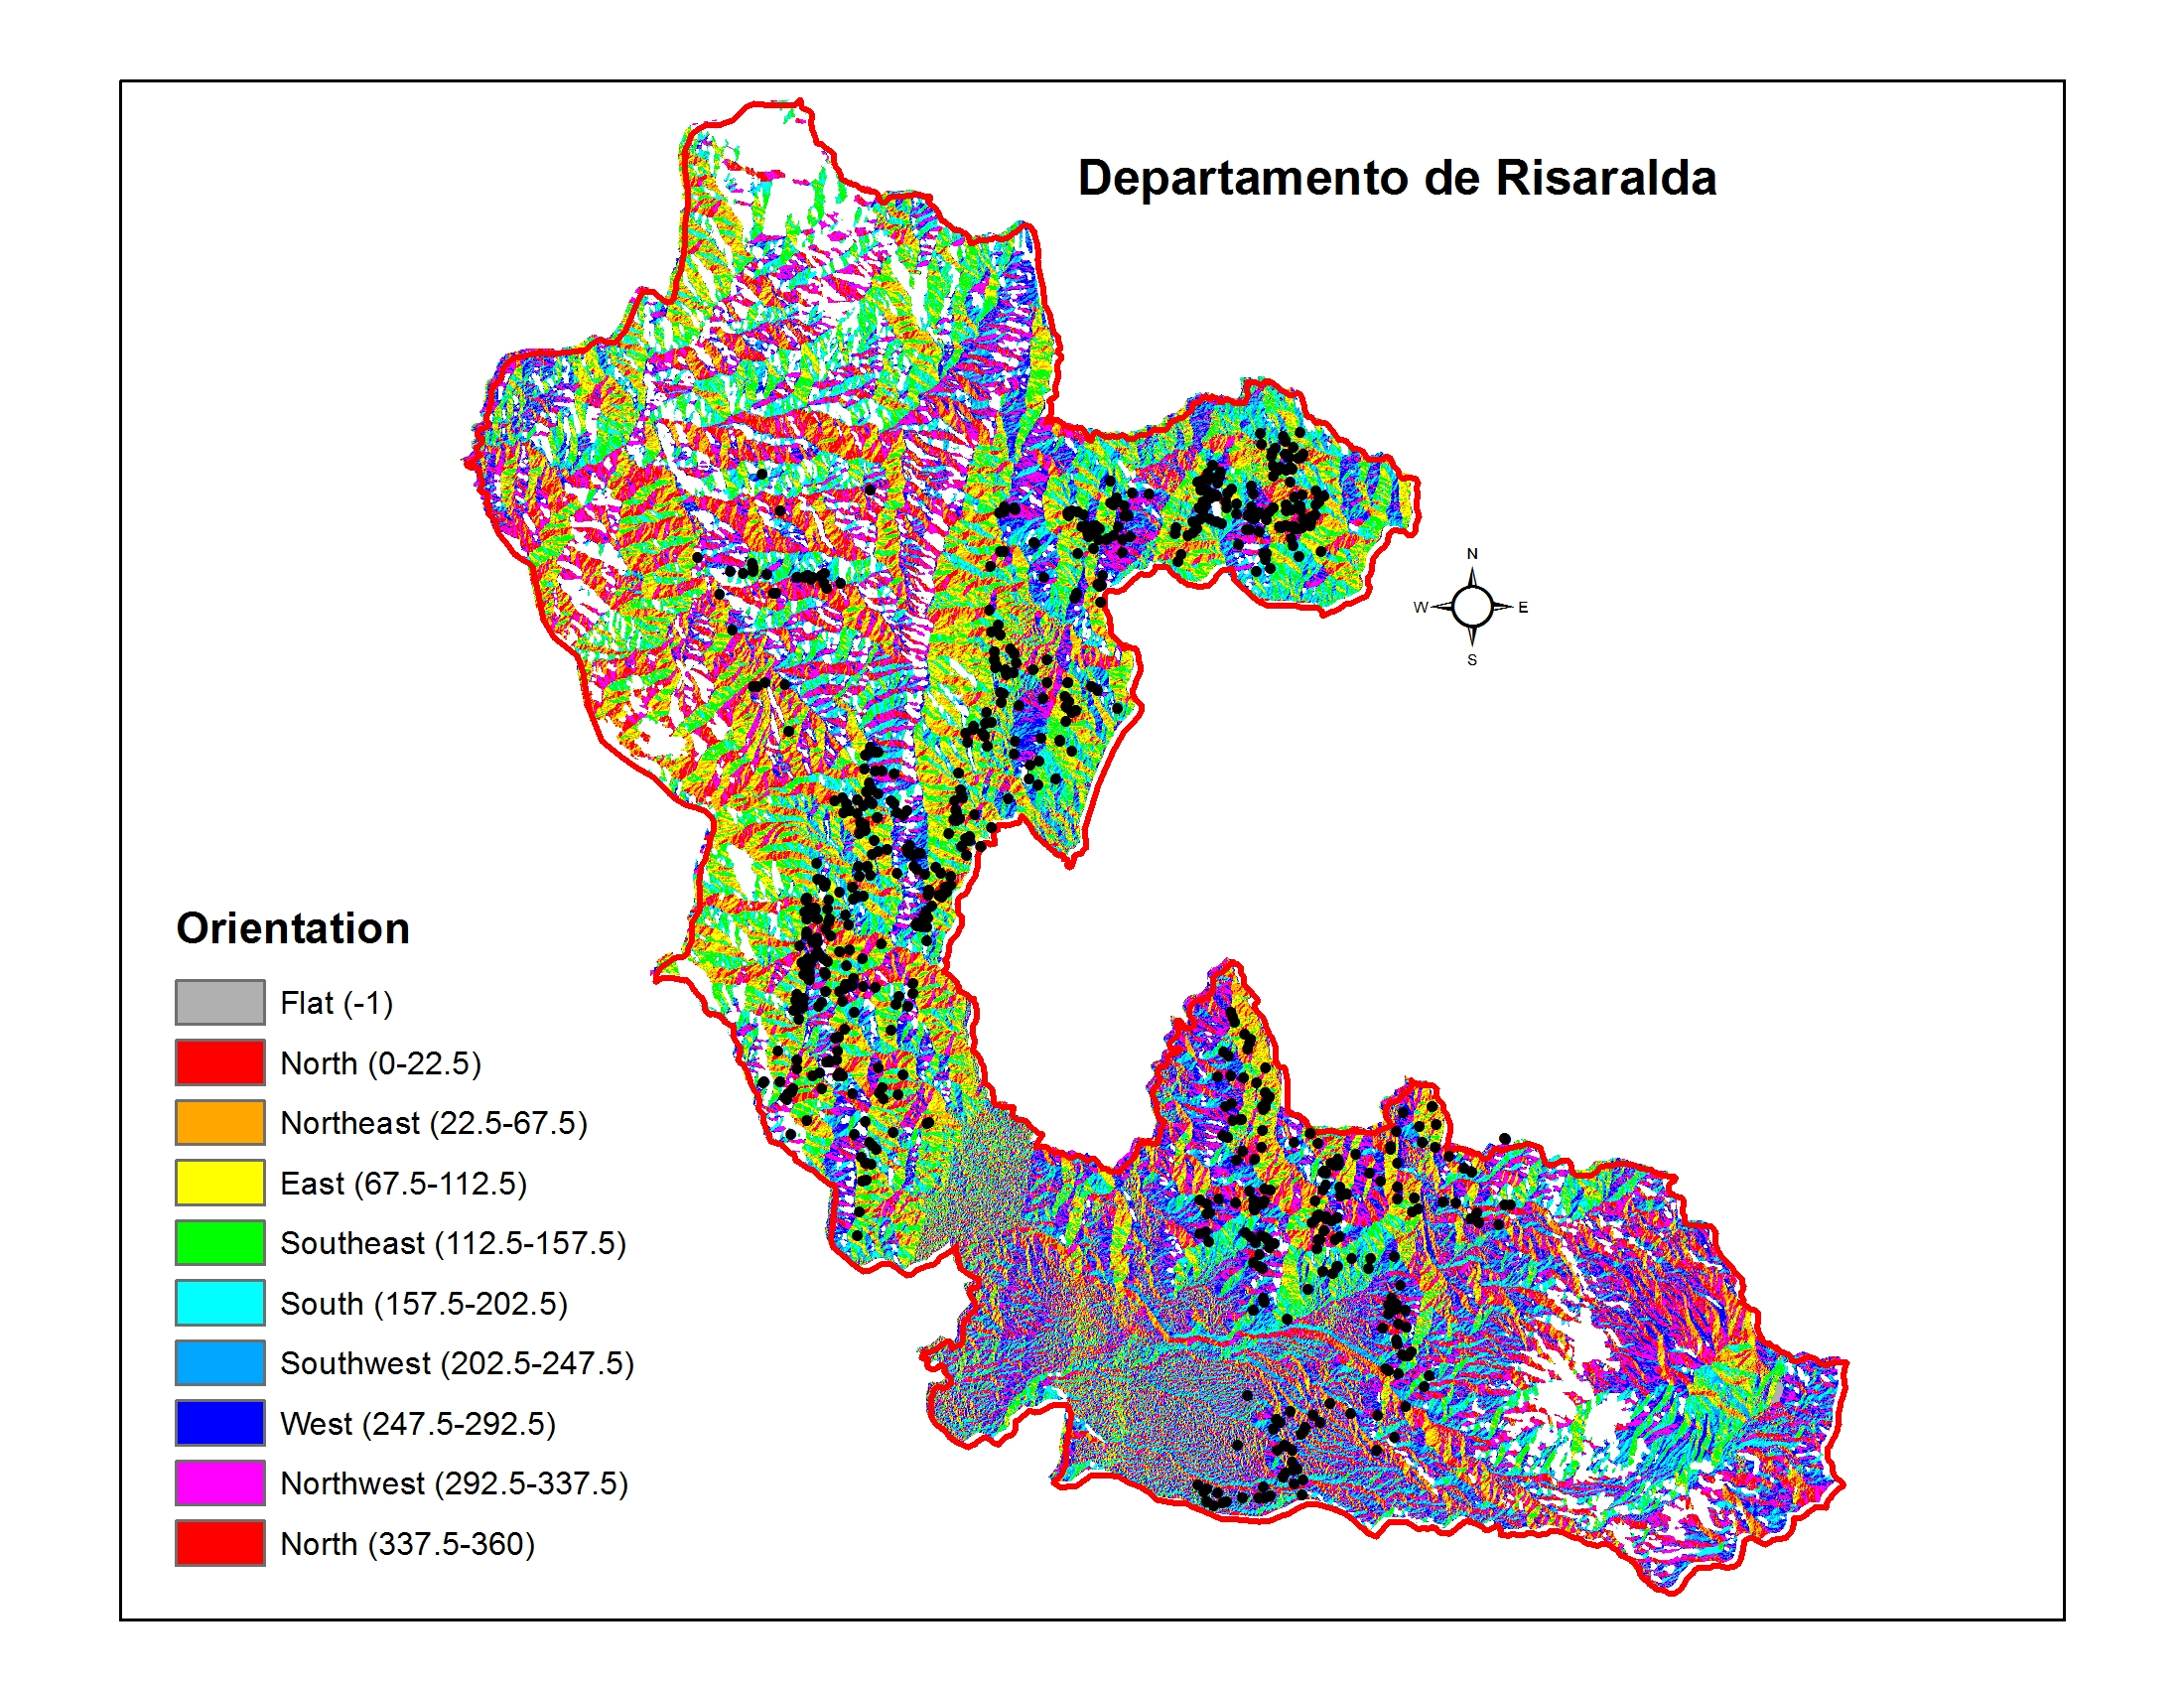
\includegraphics[width=1\linewidth]{../../Bachelor_Thesis_2017_Sources/Notebook/DataAnalysis/data/Slope_Orientation/Orientation_risaralda}
	
\end{figure}


\begin{figure}[H]
	\centering
	\caption{Shapefile des différents profils de sol dans le département de Risaralda}
	\label{fig:sigsoils}
	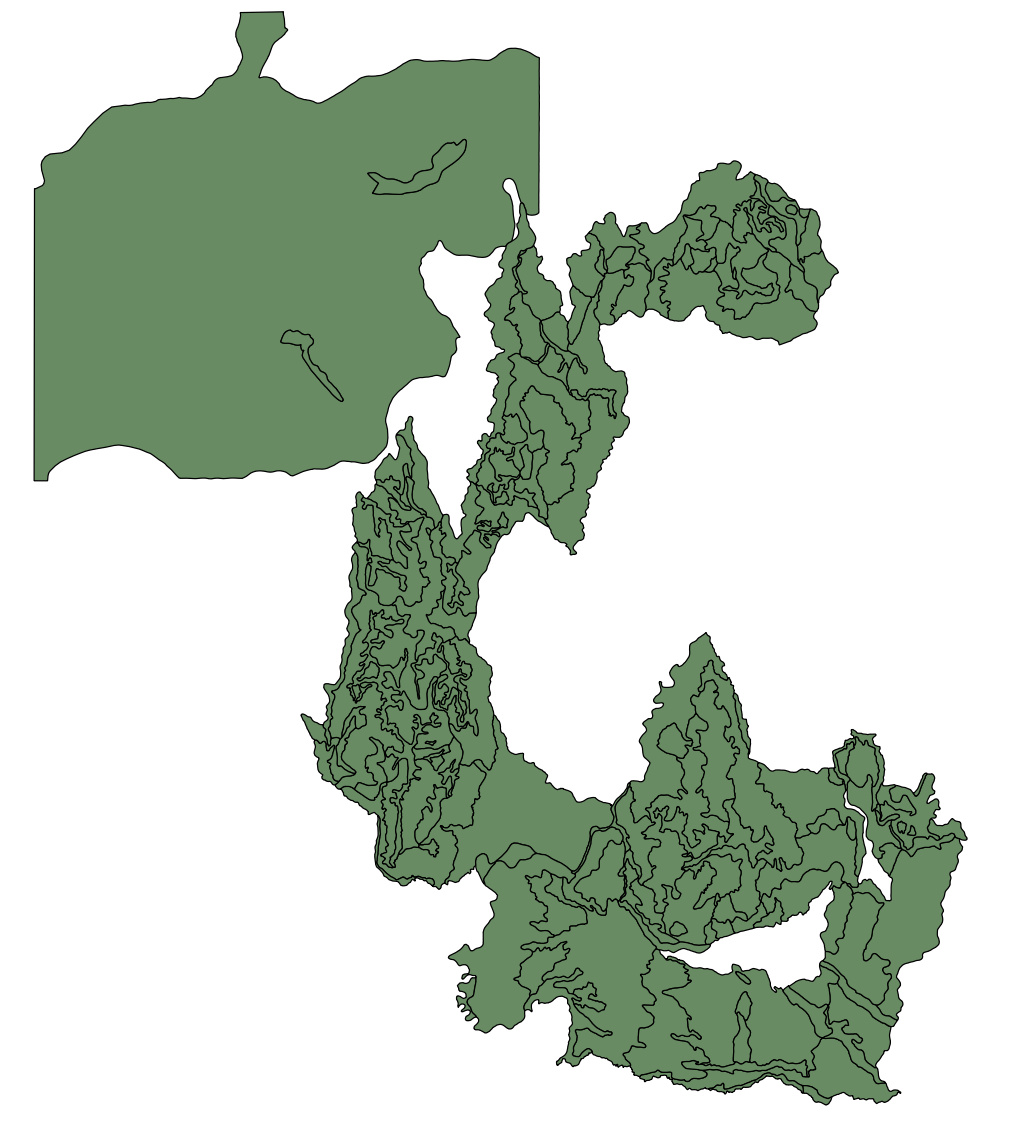
\includegraphics[width=0.7\linewidth]{img/Exploration/SIGsoils}
	
\end{figure}







\chapter{Importances des variables par cluster}
\label{annexe:clust}


\begin{table}[H]
	\centering
	\caption{HCPC avec trois clusters comparés à la sortie Acidez}
	\label{cluster3acidez}
	\begin{tabular}{llll}
		& 1  & 2  & 3   \\
		\hline
		5    & 0  & 3  & 0   \\
		5.5  & 0  & 1  & 0   \\
		6    & 3  & 6  & 18  \\
		6.25 & 1  & 1  & 3   \\
		6.5  & 5  & 8  & 35  \\
		6.75 & 1  & 0  & 7   \\
		7    & 39 & 50 & 102 \\
		7.25 & 13 & 13 & 24  \\
		7.5  & 53 & 40 & 76  \\
		7.75 & 1  & 6  & 8   \\
		8    & 0  & 59 & 47  \\
		8.25 & 0  & 8  & 4   \\
		8.5  & 0  & 1  & 0  
	\end{tabular}
\end{table}


\begin{table}[H]
	\centering
	\caption{Tableau des clusters pour la sortie Puntaje Total}
	\label{my-label}
	\begin{tabular}{llll}
		& 1  & 2  & 3  \\
		\hline
		42     & 0  & 0  & 1  \\
		49     & 0  & 1  & 2  \\
		50     & 0  & 3  & 0  \\
		52.5   & 0  & 0  & 1  \\
		58     & 0  & 0  & 1  \\
		58.5   & 0  & 1  & 0  \\
		59     & 0  & 2  & 0  \\
		59.5   & 0  & 1  & 0  \\
		60     & 0  & 3  & 2  \\
		60.5   & 0  & 2  & 0  \\
		61     & 1  & 0  & 1  \\
		61.75  & 0  & 1  & 0  \\
		62.5   & 0  & 0  & 1  \\
		63     & 0  & 1  & 0  \\
		64     & 0  & 0  & 1  \\
		65.5   & 0  & 0  & 1  \\
		66     & 0  & 1  & 1  \\
		67     & 0  & 1  & 4  \\
		68     & 1  & 0  & 2  \\
		68.75  & 0  & 1  & 0  \\
		69     & 0  & 1  & 1  \\
		69.5   & 0  & 0  & 1  \\
		69.75  & 0  & 0  & 1  \\
		70     & 0  & 0  & 1  \\
		70.75  & 1  & 0  & 0  \\
		71     & 1  & 2  & 3  \\
		71.375 & 0  & 0  & 1  \\
		71.75  & 0  & 1  & 0  \\
		72     & 0  & 1  & 2  \\
		72.5   & 0  & 1  & 0  \\
		72.75  & 0  & 0  & 1  \\
		73     & 0  & 5  & 3  \\
		73.25  & 0  & 1  & 0  \\
		73.5   & 0  & 0  & 2  \\
		74     & 0  & 0  & 2  \\
		74.75  & 0  & 1  & 1  \\
	\end{tabular}
	\begin{tabular}{llll}
		& 1  & 2  & 3  \\
		\hline
		74.875 & 0  & 0  & 1  \\
		75     & 1  & 2  & 2  \\
		75.25  & 1  & 0  & 4  \\
		75.375 & 0  & 0  & 1  \\
		75.5   & 1  & 3  & 2  \\
		75.75  & 0  & 1  & 2  \\
		76     & 2  & 2  & 8  \\
		76.125 & 0  & 0  & 2  \\
		76.25  & 0  & 0  & 2  \\
		76.375 & 1  & 0  & 0  \\
		76.5   & 4  & 3  & 6  \\
		76.75  & 1  & 0  & 4  \\
		77     & 4  & 3  & 8  \\
		77.25  & 0  & 1  & 2  \\
		77.5   & 1  & 0  & 3  \\
		77.75  & 1  & 2  & 5  \\
		77.875 & 1  & 0  & 0  \\
		78     & 7  & 4  & 3  \\
		78.25  & 0  & 1  & 1  \\
		78.5   & 1  & 1  & 7  \\
		78.75  & 0  & 0  & 2  \\
		79     & 13 & 10 & 41 \\
		79.25  & 1  & 3  & 5  \\
		79.45  & 0  & 0  & 1  \\
		79.5   & 0  & 2  & 4  \\
		79.52  & 0  & 0  & 1  \\
		79.625 & 0  & 0  & 2  \\
		79.75  & 0  & 1  & 1  \\
		80     & 6  & 7  & 8  \\
		80.25  & 0  & 1  & 4  \\
		80.375 & 0  & 0  & 1  \\
		80.5   & 2  & 1  & 8  \\
		80.625 & 1  & 0  & 0  \\
		80.75  & 1  & 2  & 8  \\
		81     & 4  & 0  & 6  \\
		81.25  & 1  & 3  & 6  \\
	\end{tabular}
	\begin{tabular}{llll}
		& 1  & 2  & 3  \\
		\hline
		81.375 & 1  & 0  & 1  \\
		81.5   & 3  & 3  & 8  \\
		81.625 & 1  & 0  & 1  \\
		81.75  & 1  & 1  & 9  \\
		82     & 7  & 4  & 13 \\
		82.25  & 7  & 2  & 4  \\
		82.375 & 2  & 0  & 2  \\
		82.5   & 29 & 24 & 19 \\
		82.75  & 5  & 3  & 4  \\
		83     & 0  & 10 & 14 \\
		83.25  & 0  & 3  & 5  \\
		83.5   & 1  & 7  & 6  \\
		83.75  & 0  & 3  & 3  \\
		84     & 0  & 5  & 8  \\
		84.25  & 0  & 5  & 2  \\
		84.5   & 0  & 8  & 5  \\
		84.75  & 0  & 6  & 1  \\
		85     & 0  & 7  & 6  \\
		85.25  & 0  & 4  & 0  \\
		85.5   & 0  & 1  & 2  \\
		85.75  & 0  & 3  & 4  \\
		86     & 0  & 4  & 1  \\
		86.25  & 0  & 0  & 1  \\
		86.5   & 0  & 3  & 2  \\
		86.75  & 0  & 1  & 3  \\
		87     & 0  & 1  & 2  \\
		87.25  & 0  & 2  & 0  \\
		87.5   & 0  & 1  & 0  \\
		87.75  & 0  & 1  & 0 \\
		&&&  \\
		&&&  \\
		&&&  \\
		&&&  \\
		&&&  \\
		&&&  \\
		&&&  
	\end{tabular}
	
\end{table}

\begin{table}[H]
	\centering
	\label{ClusterVarImp}
	\caption{Importance des variables lors de la réalisation des clusters}
	\begin{tabular}{lll}
		& Eta2       & P-value       \\
		\hline
		TmaxTotalAvg   & 0.79323282 & 8.808042e-216 \\
		TmaxTotal      & 0.79323282 & 8.808042e-216 \\
		tmean6         & 0.79308656 & 1.101237e-215 \\
		tmax6          & 0.77941800 & 6.561977e-207 \\
		TmeanTotalAvg  & 0.77802701 & 4.779121e-206 \\
		TmeanTotal     & 0.77802701 & 4.779121e-206 \\
		tmax7          & 0.77433881 & 8.706622e-204 \\
		tmean10        & 0.77341542 & 3.162373e-203 \\
		tmean5         & 0.77255468 & 1.047399e-202 \\
		tmean7         & 0.77146031 & 4.770308e-202 \\
		tmean9         & 0.76659843 & 3.682110e-199 \\
		tmax5          & 0.75947622 & 4.888995e-195 \\
		tmean8         & 0.75943990 & 5.127819e-195 \\
		tmax8          & 0.75506157 & 1.527633e-192 \\
		tmax9          & 0.73797359 & 2.717166e-183 \\
		tmin10         & 0.73685898 & 1.038321e-182 \\
		tmean4         & 0.72591249 & 4.041247e-177 \\
		tmax1          & 0.72445394 & 2.159972e-176 \\
		tmax4          & 0.72115391 & 9.274507e-175 \\
		tmax10         & 0.71764667 & 4.803959e-173 \\
		tmean1         & 0.71497543 & 9.398029e-172 \\
		tmin6          & 0.70461972 & 7.372790e-167 \\
		TminTotalAvg   & 0.68401310 & 1.306441e-157 \\
		TminTotal      & 0.68401310 & 1.306441e-157 \\
		tmean2         & 0.67984980 & 8.149567e-156 \\
		tmin8          & 0.67467087 & 1.293430e-153 \\
		tmax2          & 0.66718704 & 1.700396e-150 \\
		tmin9          & 0.66714064 & 1.776914e-150 \\
		tmean3         & 0.66366823 & 4.707493e-149 \\
		tmin7          & 0.65549751 & 9.209679e-146 \\
		tmax3          & 0.64170621 & 2.220623e-140 \\
		tmin5          & 0.63104980 & 2.317687e-136 \\
	\end{tabular}
\end{table}
\newpage
\begin{table}[H]
	\centering
	\label{ClusterVarImp2}
	\begin{tabular}{llll}
		& Eta2       & P-value       \\
		\hline
		tmin3          & 0.61739273 & 2.231189e-131 \\
		tmin4          & 0.61250703 & 1.225099e-129 \\
		tmin1          & 0.61199847 & 1.853488e-129 \\
		tmin2          & 0.60842700 & 3.343356e-128 \\
		DtrTotalAvg    & 0.55204696 & 9.200736e-110 \\
		DtrTotal       & 0.55204696 & 9.200736e-110 \\
		prec10         & 0.52838295 & 1.045148e-102 \\
		PrecTotalAvg   & 0.51318493 & 2.320750e-98  \\
		PrecTotal      & 0.51318493 & 2.320750e-98  \\
		ASNM           & 0.50548203 & 3.287540e-96  \\
		prec6          & 0.48690365 & 3.716337e-91  \\
		dtr8           & 0.47172566 & 3.664625e-87  \\
		prec4          & 0.46275569 & 7.423006e-85  \\
		dtr1           & 0.45506364 & 6.575620e-83  \\
		prec5          & 0.43486454 & 6.354576e-78  \\
		dtr7           & 0.43333703 & 1.488559e-77  \\
		dtr10          & 0.42305017 & 4.330758e-75  \\
		dtr2           & 0.41092218 & 3.056574e-72  \\
		dtr4           & 0.39912083 & 1.589035e-69  \\
		dtr5           & 0.39851482 & 2.183452e-69  \\
		dtr6           & 0.38517429 & 2.199730e-66  \\
		dtr9           & 0.38032942 & 2.611213e-65  \\
		dtr3           & 0.32744102 & 4.212873e-54  \\
		prec7          & 0.27997934 & 8.894746e-45  \\
		prec9          & 0.27175535 & 3.172161e-43  \\
		prec3          & 0.26360964 & 1.050396e-41  \\
		prec1          & 0.12139964 & 1.224259e-17  \\
		prec8          & 0.11382522 & 1.787707e-16  \\
		prec2          & 0.10476930 & 4.266965e-15  \\
		Luminosidad    & 0.03438122 & 6.133050e-05  \\
		Arcilloso      & 0.02674672 & 6.590146e-04  \\
		OrientationNum & 0.02251785 & 2.402284e-03  \\
		Limoso         & 0.01764046 & 1.041358e-02  \\
		pH\_avg        & 0.01665250 & 1.395976e-02  \\
		Cascajoso      & 0.01553506 & 1.940861e-02  \\
		Franco         & 0.01291747 & 4.161129e-02 
	\end{tabular}
\end{table}















\chapter{Autres informations \label{annexeAutre}}
%TODO -> noter les URLS
\noindent Les sources du projet se trouvent sur un dépot \textit{Github} à l'adresse \url{https://github.com/ThibaultSchowing/Bachelor_Thesis_2017_Sources}.\\


\noindent Le présent document et les fichiers associés se trouvent sur un dépot \textit{Github} à l'adresse \url{https://github.com/ThibaultSchowing/Bachelor_Thesis_2017}.\\



\noindent Les partial plots sont disponibles sur le dépot \textit{Github} du projet à l'adresse \url{https://github.com/ThibaultSchowing/Bachelor_Thesis_2017_Sources/tree/master/Notebook/R/Projects/BachelorThesis/PartialPlots}. \\


\noindent Les analyses par variétés sont disponible sur le dépot \textit{Github} du projet à l'adresse \url{https://github.com/ThibaultSchowing/Bachelor_Thesis_2017_Sources/tree/master/Notebook/R/Projects/BachelorThesis/VARIETY_ANALYSIS}. Les répertoires créés ne sont pas forcément représentatifs des analyses effectuées et peuvent être vides. \\





















